% !TEX root =  paper.tex

\section{Background and Motivating Example}
\label{sec:background}
\Cref{fig:motivating-example} shows an example
of a web page with overlaid segments (marked as green boxes).
As can be seen from the figure,
the segments divide the page into a set 
of coherent groups.
Coherency in this context indicates a perceptual grouping of related elements,
where a user is able to intuitively recognize that
a page is composed of a group of segments.
For instance, in \Cref{fig:motivating-example},
a user can intuitively divide the page into 
a set of segments, such as a top/header segment, a main content segment,
and a footer segment. 

Web page segmentation is used in various areas of software engineering.
Saar et al.~\cite{saar2016browserbite}
use segmentation to test
cross-browser compatibility of web pages.
Their approach is based on
loading the same web page in two different browsers,
followed by segmenting the rendered pages in the two different browsers,
and finally comparing the pairs of segments
to ensure both pages have been rendered
in the same fashion in both browsers. 
A similar technique is used by Huse et al.~\cite{huse2008using}.
Mahajan et al.~\cite{mahajan2018automated}
propose an approach to automatically test and repair mobile layout bugs.
They first perform a segmentation of the  page to localize bugs.
Each segment is then passed to an oracle that reports a list of layout bugs.
Finally, the segment's CSS code is then patched based on a list of database patches.
A similar analysis is used for testing and repairing
web page internationalization bugs~\cite{mahajan2018automated_intl}.
Page segmentation has also been used in security testing.
Geng et al.~\cite{geng2015combating} propose a segmentation-based 
approach to detect phishing security attacks.
Their technique extracts segments from a page, and then uses
the segments to extract features, build a fingerprint of the page, 
and detect whether a page under test is phishing.

The segments shown in \Cref{fig:motivating-example} can be generated using
a number of techniques, as described in the following subsections.

\subsection{DOM-based Page Segmentation}
One approach is to use information based on the Document Object Model (DOM)~
\cite{rajkumar2012dynamic,vineel2009web,kang2010repetition}.
This approach utilizes the DOM tags, attributes, or subtrees for its analysis,
after which a set of thresholds are applied to generate a subset of DOM elements
representing the final extracted segments.
For instance, Rajkumar et al.~\cite{rajkumar2012dynamic} propose an algorithm based
on detecting tag name repetitions in the DOM.
It represents each DOM element as a string of tag names in a similar fashion
to XPaths. It then detects repeating substrings.
These repetitions (of a certain length and a certain occurrence threshold)
would then be considered web page segments.
Vineel et al.~\cite{vineel2009web} 
analyzes the DOM by first thresholding elements containing more than a certain number
of child node characters, followed by thresholding elements with more repetitive
children tag names. The rationale being that elements containing more uniform tag name
repetitions are more likely to represent a page structure.
The set of thresholded elements are then taken as the page segments.

DOM approaches, however, focus exclusively on the tag tree structure
and therefore not directly related
to what the user is actually perceiving on screen.
That is, the analysis is conducted on the tree structure by checking a set of
rules or relationships between various nodes, parents, and children.
This tree structure and the various rules and relationships between nodes
are not directly related to the final visual rendering perceived by the user.

\begin{figure}
    \centering
    {%
    \setlength{\fboxsep}{0pt}%
    \setlength{\fboxrule}{1pt}%
    \fbox{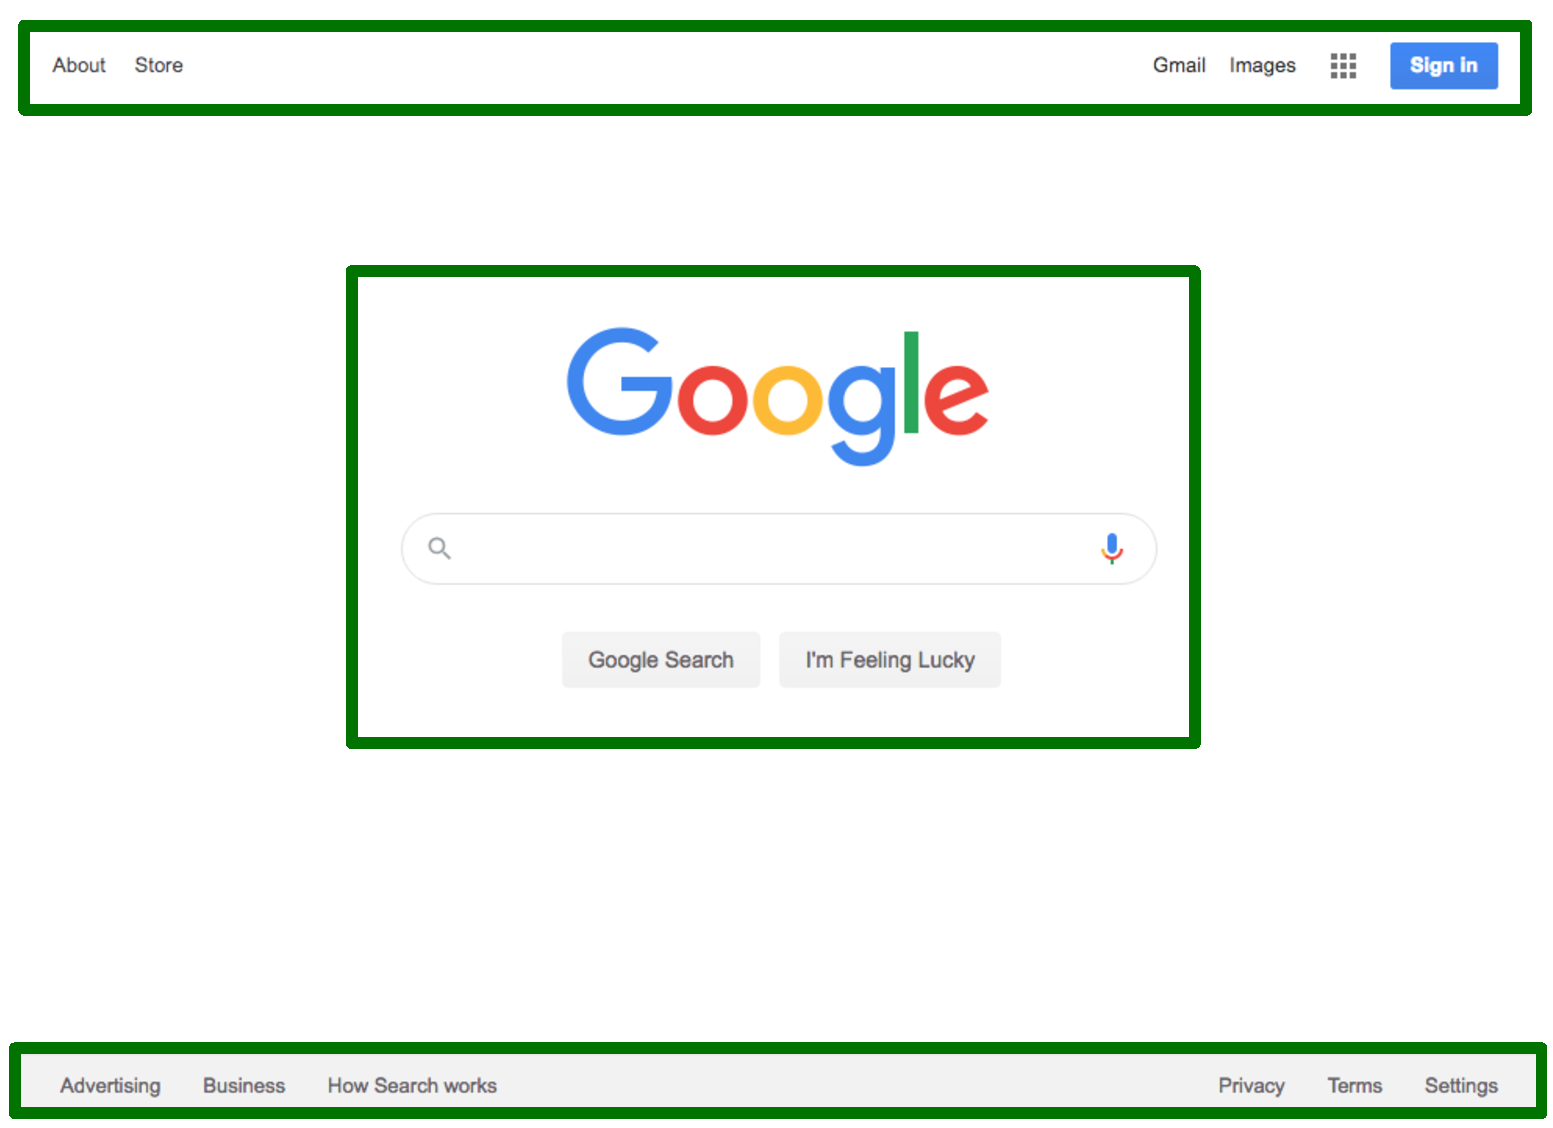
\includegraphics[trim=0 0 0 0,clip,scale=0.31]{figures/motivating-example/motivating-example.pdf}}
    }%
    \caption{An example of web page segmentation.
    Green boxes indicate detected page segments.}
    \label{fig:motivating-example}
\end{figure}

\subsection{Text-based Page Segmentation}
A number of alternative approaches were proposed to explore complementary
ways by which the generated segments can be made more accurate and meaningful.
One such alternative approach relies on the use of text-based algorithms~
\cite{kohlschutter2008densitometric, kolcz2007site}.
This form of segmentation analyzes the textual content of
the page as opposed to the DOM tree structure.
For instance, Kohlsch{\"u}tter et al.~\cite{kohlschutter2008densitometric} divide the page into a set of text blocks.
Each block is a continuous piece of text, potentially spanning multiple tags.
The approach then computes text density, a common measure from the field of 
quantitative linguistics. It is computed by dividing the number of text tokens
by the number of lines. This is done for each text block.
Whenever two consecutive blocks have a text density difference below a certain threshold,
the blocks are merged together. This process is repeated and the resultant
blocks are taken as the page segments.
Kolcz et al.~\cite{kolcz2007site} propose an approach that first selects the text
child nodes in a predefined set of tags (e.g., \code{<table>}, \code{<div>}, \code{<blockquote>}). This excludes
certain tags that are not likely to contain significant textual information (e.g., \code{<b>}, \code{<u>}).
Next, selection is reduced to a set of text nodes that have at least
40 characters and three different types of textual tokens (e.g., nouns, verbs).
The resulting set of text blocks are taken as the final page segments.

While text-based approaches do consider an aspect of the page that is more
perceptible by the end user (i.e., the text and its characteristics),
they ignore many aspects of the page such as structure, styles, layout, and images.


\subsection{Visual Page Segmentation}
Another approach considers visual attributes of the page.
Cai et al.~\cite{cai2003vips} propose
the VIPS (\textbf{Vi}sion-based \textbf{P}age \textbf{S}egmentation)
algorithm, a quite popular state-of-the-art page segmentation tool~\cite{sleiman2013survey, campus2011web}.
The approach begins at the root DOM node.
It then iteratively splits the page to smaller segments.
Splitting is based on many hard-coded rule sets.
For example, one rule is that if a DOM node has an \code{<hr>} child, 
which represents a horizontal line,
then divide it in two (at the \code{<hr>} child) . 
The approach contains many similar hard-coded rules, 
but this makes it less robust due to assuming that developers always 
use certain tags in the same pre-defined way, which is not always true.
The approach also requires a number of thresholds,
such as a \emph{coherence threshold} that indicates whether a segment is coherent,
as well as thresholds on the dimensions of segments (e.g., width, height), among others.
Requiring many parameters from the user increases manual effort and 
often reduces accuracy due to sub-optimal parameter tuning and overfitting.

Note that the VIPS approach, despite its name, is actually not vision-based
in the sense that it does not perform visual analyses
from a computer vision perspective,
such as visually analyzing the overall visual structure of the page.
Rather, most of the analyses conducted in VIPS rely heavily on the DOM tree structure.
It was referred to as vision-based because, in some of its stages,
it uses DOM attributes that are visual in nature,
such as background color and element size.
If we envision a spectrum of techniques with DOM-based segmentation on one end
and visual segmentation on the other end, VIPS would be closer to a
DOM-based segmentation.

Visual techniques can also be at a disadvantage in some tasks. For instance, visually identifying
text blocks (i.e., via OCR - optical character recognition) can sometimes be 
inaccurate and remains an active area of research in computer vision.
On the other hand, the same task (i.e., text block identification) 
is more readily available and accessible from the DOM, 
and therefore DOM-based approaches would be more reliable in this case. 

